\subsection{Fuel salt reprocessing system}

\begin{frame}
  \frametitle{Fuel salt reprocessing system overview: gas separation}
  Gaseous fission products (e.g., Xe, Kr) must be removed from the fuel salt 
  to avoid reactor poisoning ($\Sigma_{a,^{135}Xe}=10^6\dots10^7$b). 
  
      \begin{columns}
      	\column[t]{4.0cm}
    \begin{block}{Noble gas removal}
      \begin{enumerate}
      	\item[\textcolor{blue}{\textbullet}] bubble generator injects He 
      	bubbles in the salt stream
      	\item[\textcolor{green}{\textbullet}] noble gas migrate to the He 
      	bubbles 
      	\item[\textcolor{red}{\textbullet}] gas separator discharges the 
      	poison-rich bubbles
      \end{enumerate}
    \end{block}    	
      	
     	\column[t]{8cm}
  \begin{figure}[t]
	  \centering
	  		\vspace{-1mm}
		\includegraphics[width=\textwidth]{./images/msbr_gas_separation.pdf}
	\caption{Schematic flow diagram of the \gls{MSBR} gas separation system 
	(figure reproduced from Robertson \emph{et al.}  
	\cite{robertson_conceptual_1971}).} 
    \end{figure}

	\end{columns}
\end{frame}

\begin{frame}
  \frametitle{Mathematical model for gas separation efficiency}
  		\vspace{-1mm}
Xenon removal efficiency ($\epsilon_{Xe}$) in a gas separation system is 
\cite{peebles_removal_1968, sada_gas-liquid_1987}:
\begin{align}
& \qquad\qquad \epsilon_{Xe} = \frac{1-e^{-\beta}}{1+\alpha} \nonumber \\
\alpha &= \frac{RTQ_{L}}{HQ_{G}} \nonumber \\
\beta &= K_L \frac{6}{d_b} \frac{Q_G}{Q_G+G_L} \frac{A_C L (1+\alpha)}{Q_{L}} 
\nonumber \\
Q_{L}&= \mbox{volumetric salt flow rate [$m^3/s$]} \nonumber \\
Q_{G}&= \mbox{volumetric helium flow rate [$m^3/s$]} \nonumber \\
H &= \mbox{Henry's law constant [$Pa\cdot mol^{-1}\cdot L$]} \nonumber \\
d_b &= \mbox{helium bubble diameter [m]} \nonumber \\
K_L &= \mbox{liquid phase mass transfer coefficient [m/s].} \nonumber
\end{align}
		\vspace{-6mm}
  \begin{figure}[t]
	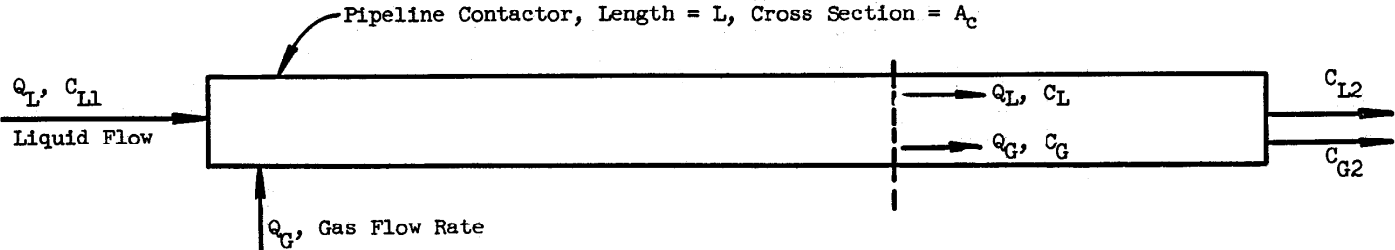
\includegraphics[width=0.66\textwidth]{./images/pipeline_contactor.png}
	\vspace{-3mm}
	\caption{Flow diagram for gas separator (figure reproduced from Peebles 
		\emph{et al.} \cite{peebles_removal_1968}).}
\end{figure}

\end{frame}


%\begin{frame}
%\frametitle{Fuel processing system overview: rare earths and Pa removal}
%		\vspace{-2mm}
%	\begin{figure}[htp!] % replace 't' with 'b' to 
%		\centering
%			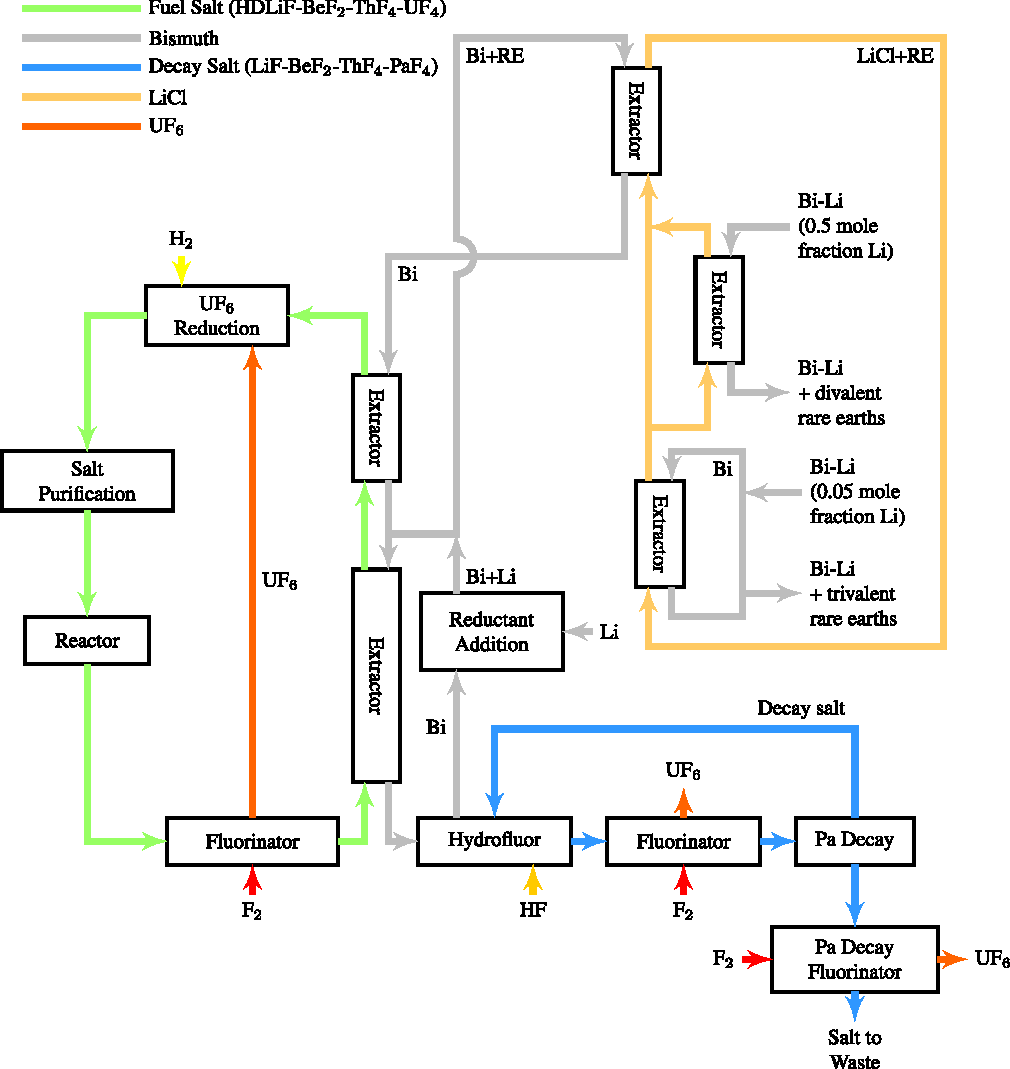
\includegraphics[width=0.57\textwidth]{../figures/flowsheet.pdf}
%			\vspace{-2mm}
%		\caption{Liquid metal (Bi) extraction system for the \gls{MSBR} 
%		(reproduced from Sorensen \cite{sorensen_one-fluid_2006}).} 
%	\end{figure}
%\end{frame}


\begin{frame}
\frametitle{Fuel processing system overview: TAP concept}
	\vspace{-2mm}
\begin{figure}[htp!] % replace 't' with 'b' to 
	\centering
	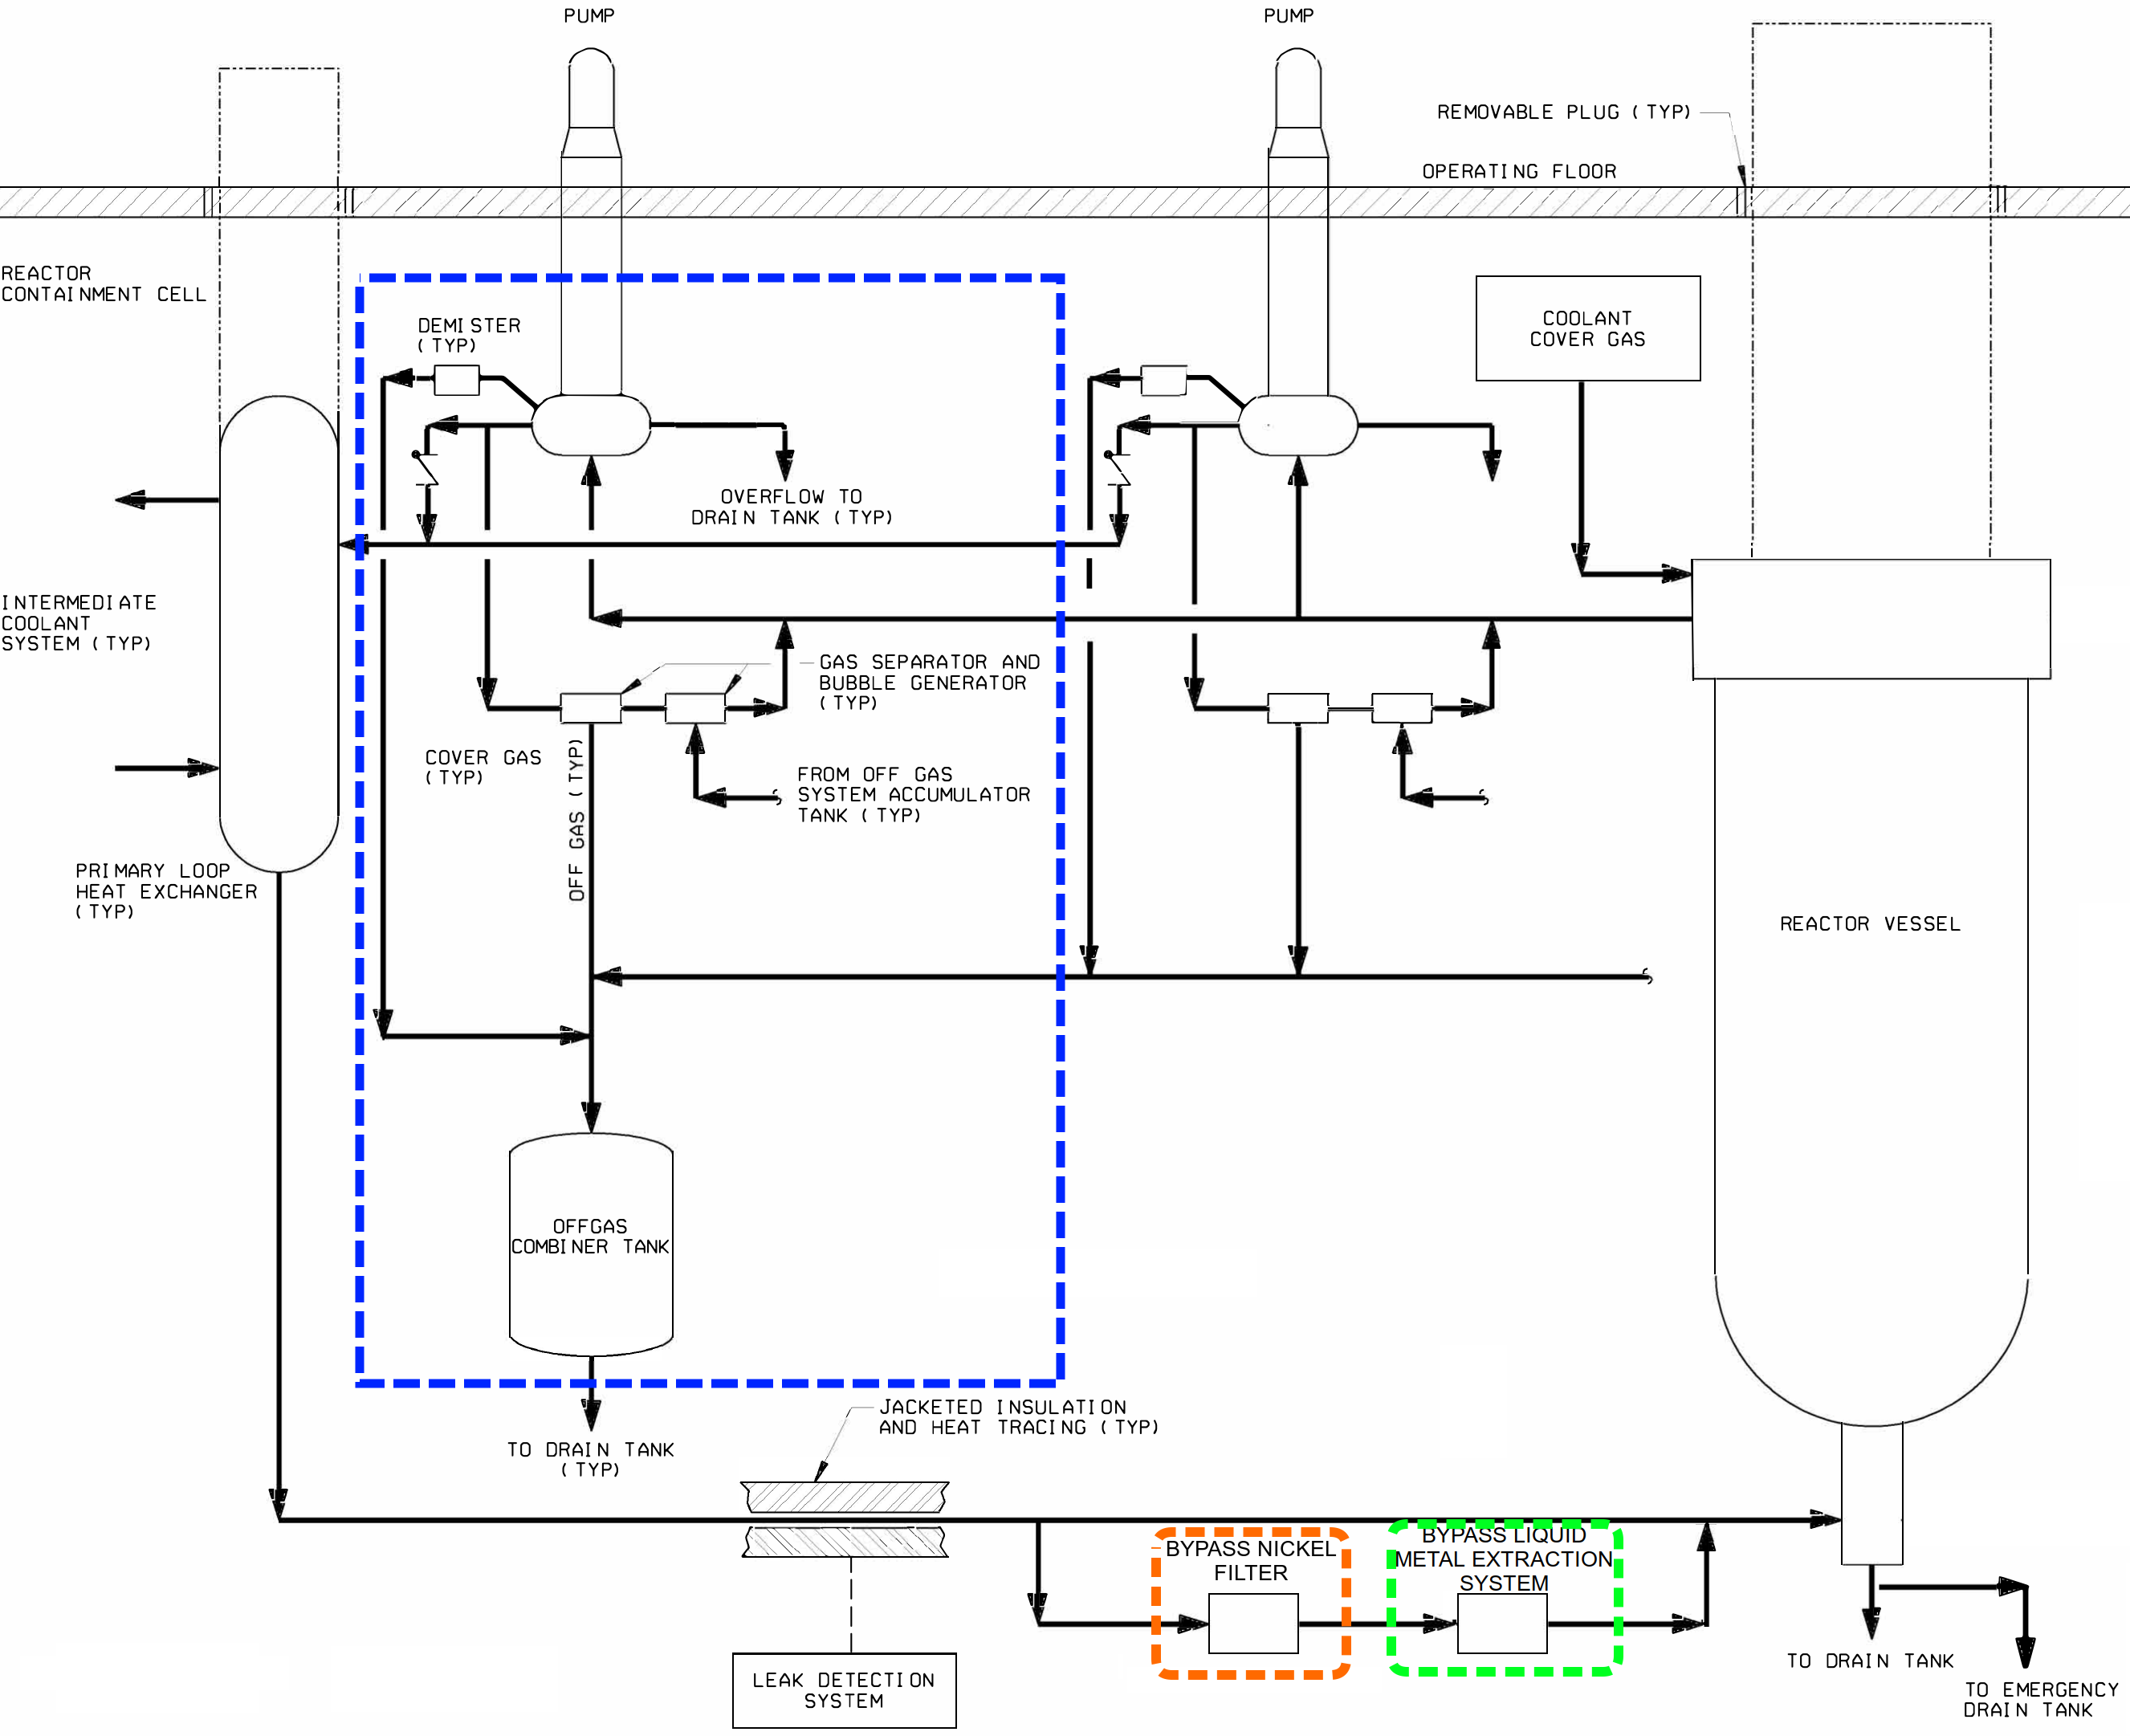
\includegraphics[width=0.75\textwidth]{../dissertation/figures/ch4/tap_primary_loop.png}
		\vspace{-2mm}
	\caption{Simplified \gls{TAP} primary loop design including off-gas system 
		(blue), nickel filter (orange) and liquid metal extraction system 
		(green) \cite{transatomic_power_transatomic_2019}.}
\end{figure}

\end{frame}

\begin{frame}
\frametitle{SaltProc demonstration for TAP concept input data}
\begin{textblock*}{12.5cm}(0.5cm,1.6cm) % {block width} (coords)
	%%%%%%%%%%%%%%%%%%%%%%%%%%%%%%%%%%%%%%%%
	\begin{table}[htbp!]
		\fontsize{6}{9}\selectfont
		\centering
		\caption{The effective cycle times and rates for fission products 
		removal \cite{robertson_conceptual_1971, betzler_implementation_2017}.}
			\vspace{-2mm}
		\begin{tabular}{p{0.14\textwidth} p{0.3\textwidth} p{0.11\textwidth} 
				p{0.11\textwidth}}
			\hline 
			\textbf{Processing group} & \qquad\qquad\qquad \textbf{Nuclides} & 
			\textbf{Removal Rate (s$^{-1}$)} & \textbf{Cycle time (at full 
			power)} 
			\\ \hline 
			\multicolumn{3}{c}{\textit{Elements removed in \gls{MSBR} and 
			adopted for the \gls{TAP}} 
					\cite{robertson_conceptual_1971}} \\
			Noble gases & Xe, Kr								  & 5.00E-2 & 
			20 
			sec \\
			Noble metals & Se, Nb, Mo, Tc, Ru, Rh, Pd, Ag, Sb, Te & 5.00E-2 & 
			20 
			sec \\
			Seminoble metals & Zr, Cd, In, Sn	  				  & 5.79E-8 & 
			200 
			days\\
			Volatile fluorides & Br, I 							  & 1.93E-7 & 
			60 
			days\\
			Rare earths & Y, La, Ce, Pr, Nd, Pm, Sm, Gd           & 2.31E-7 & 
			50 
			days\\
			\qquad & Eu & 2.32E-8 & 500 days \\
			Discard & Rb, Sr, Cs, Ba & 3.37E-9 & 3435 days \\
			\hline
			\multicolumn{3}{c}{\textit{Additional elements removed in 
			\gls{TAP}} 
				\cite{betzler_implementation_2017, 
					transatomic_power_corporation_neutronics_2016}} \\
			Noble gases & H								  	& 5.00E-2 & 20 
			sec    \\
			Noble metals & Ti, V, Cr, Cu						& 3.37E-9 & 
			3435 
			days \\
			Seminoble metals & Mn, Fe, Co, Ni, Zn, Ga, Ge, As   & 3.37E-9 & 
			3435 
			days \\
			Rare earths & Sc									& 3.37E-9 & 
			3435 
			days \\
			Discard & Ca										& 3.37E-9 & 
			3435 
			days \\
			\hline
			\multicolumn{3}{c}{\textit{Additional elements removed in 
			\gls{MSBR}} 
				\cite{robertson_conceptual_1971}} \\
			Protactinium & Pa  	& 3.86E-6 & 3 days    \\
			\hline
		\end{tabular}
		\label{tab:reprocessing_list}
	\end{table}
	\begin{itemize}
		\item Noble gas removal efficiency: variable, defined using 
		mathematical model
		\item Other FP removal efficiency: fixed and based on 
		Table~\ref{tab:reprocessing_list}
	\end{itemize}
\end{textblock*}
\end{frame}


\subsection{SaltProc tool design}


\begin{frame}
\frametitle{SaltProc class architecture}
	\begin{itemize}
		\item \textit{Simulation} class
			\begin{itemize}
				\item Manages simulation process
				\item Stores data into the HDF5 database
				\item Tracks time, power level
			\end{itemize}
		\item \textit{Depcode} class
			\begin{itemize}
				\item Contains attributes and methods for reading user's input
				\item Creates input files for depletion code
				\item Parses depletion code output 
			\end{itemize}
		\item \textit{Process} class
			\begin{itemize}
				\item Represents fuel processing system component
				\item Contains attributes of the component ($\vec{\epsilon}$, 
				throughput rate)
				\item Tracks waste stream
			\end{itemize}
		\item \textit{MaterialFlow} class
			\begin{itemize}
				\item Instances of that class represents the material flowing between processes
			\end{itemize}
	\end{itemize}
		\vspace{1mm}
	\begin{figure}[ht!] % replace 't' with 'b' to 
		\centering
		\begin{overprint}
		\onslide<1>\centerline{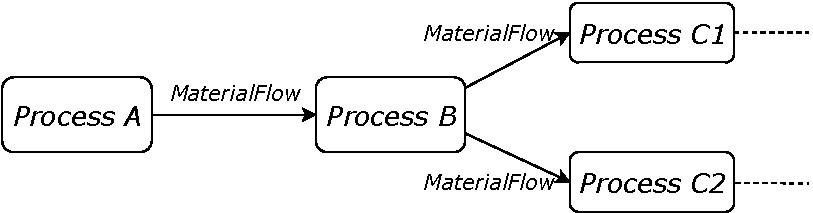
\includegraphics[width=0.6\textwidth]{../dissertation/figures/ch2/materialflow.pdf}}
		\onslide<2>\centerline{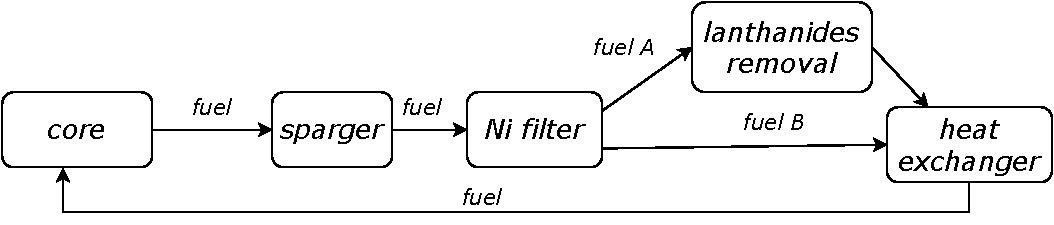
\includegraphics[width=0.6\textwidth]{../dissertation/figures/ch2/tap_materialflow.pdf}}
		\end{overprint}
		\vspace{-2mm}
		\caption{Schematic for passing material data between fuel processing 
		system components.}
	\end{figure}

\end{frame}


\begin{frame}
\frametitle{SaltProc flowchart}
\vspace{-4mm}
\begin{figure}[ht!] % replace 't' with 'b' to \centering
	\centering
	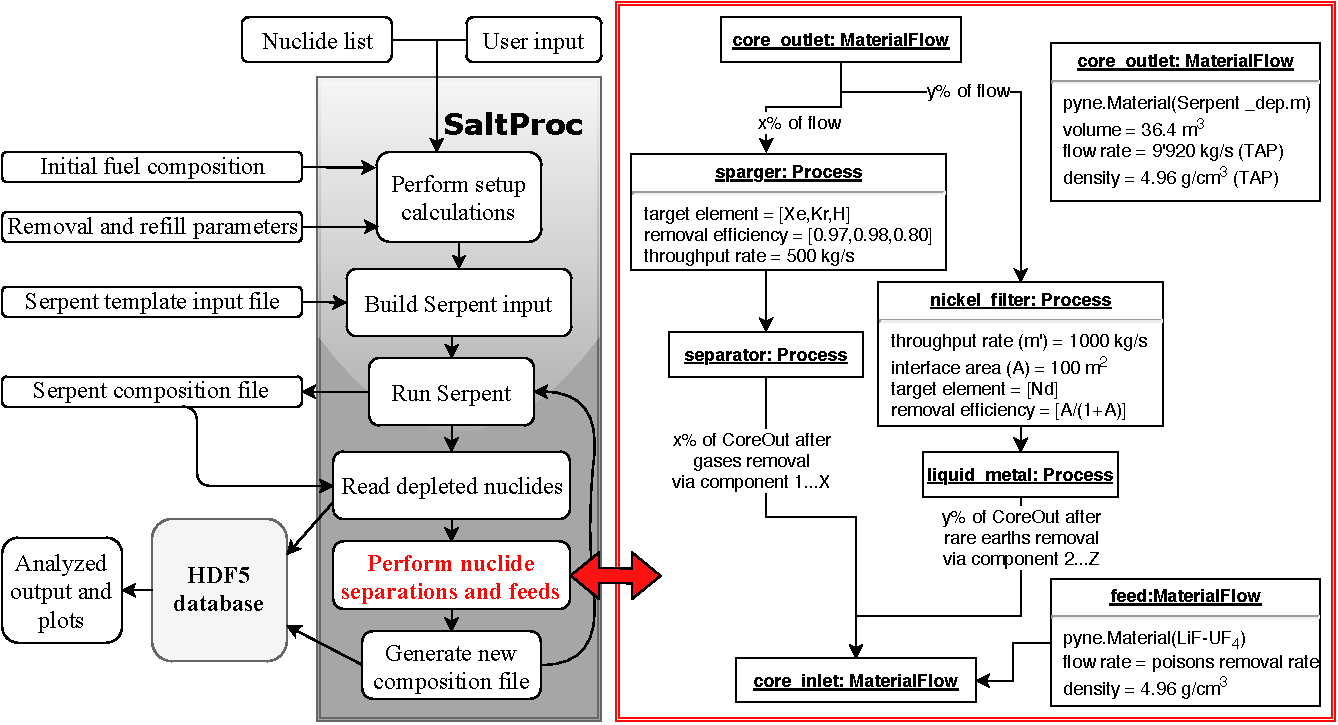
\includegraphics[width=1.08\textwidth]{../dissertation/figures/ch2/saltproc_flowchart.pdf}
		\vspace{-4mm}
	\caption{SaltProc v1.0 Python package flowchart.}
\end{figure}

\end{frame}


\begin{frame}
\frametitle{Multi-component fuel reprocessing system model in SaltProc}       

\begin{figure}[htp!] % replace 't' with 'b' to 
	\centering
	\vspace{-2mm}
	\begin{overprint}
	\onslide<1>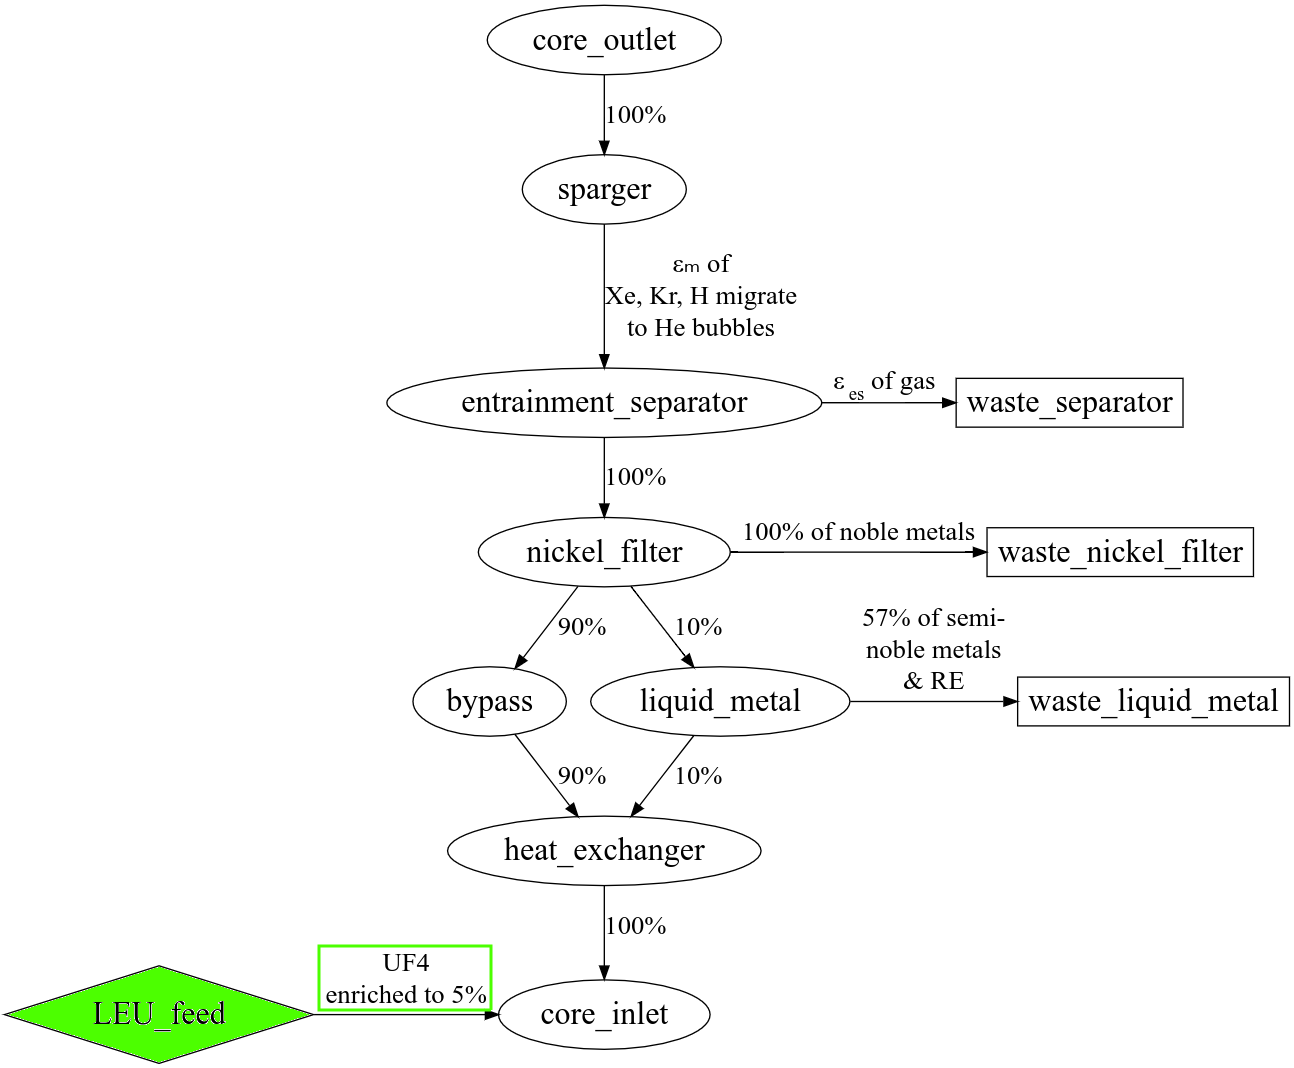
\includegraphics[height=0.85\textheight]{./images/tap_saltproc_var_eps.png}
		\vspace{-2mm}
    \caption{\textcolor{green}{\gls{TAP}} reprocessing scheme for 
	SaltProc demonstration.}
	\onslide<2>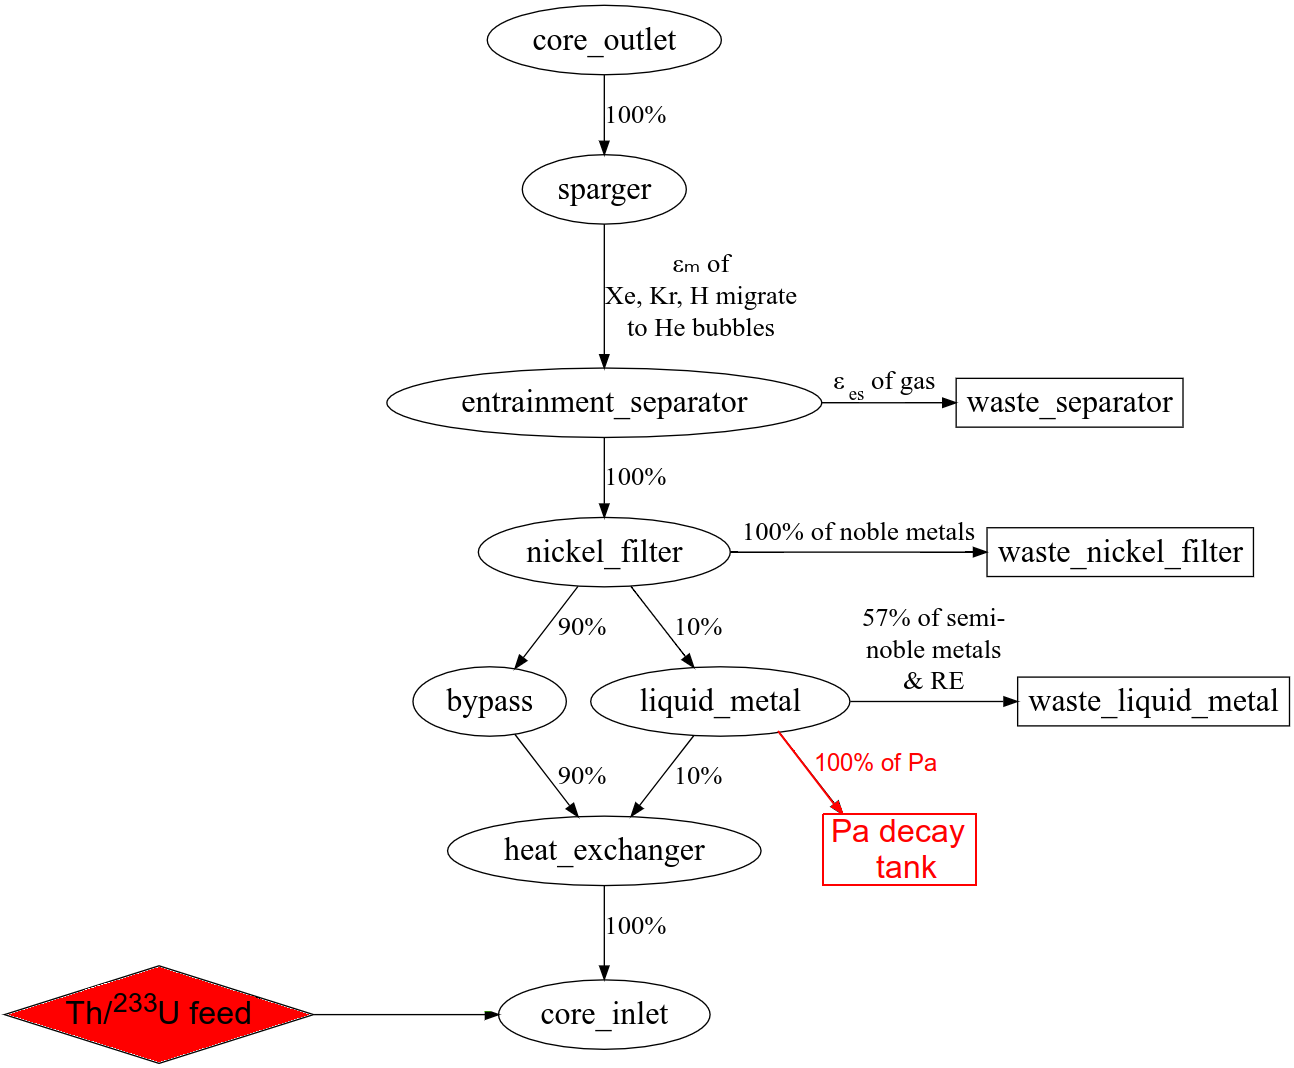
\includegraphics[height=0.85\textheight]{./images/msbr_saltproc_var_eps.png}
		\vspace{-2mm}
	\caption{\textcolor{red}{\gls{MSBR}} reprocessing scheme for 
	SaltProc demonstration.}
	\end{overprint}
\end{figure}

\end{frame}


\begin{frame}[fragile]
\frametitle{DOT code used to describe TAP reprocessing system}
\small
\begin{verbatim}
digraph fuel {
==============================================================================
core_outlet -> sparger [label="100%", fontsize=20]
sparger -> waste_sparger [label="60% of\nXe, Kr, H", fontsize=20]
sparger -> entrainment_separator [label="100%", fontsize=20]
entrainment_separator -> nickel_filter [label="100%", fontsize=20]
entrainment_separator -> waste_entrainment_separator [label="97% of\nXe, Kr, 
%H", fontsize=20]
nickel_filter -> bypass [label="90%", fontsize=20]
bypass -> heat_exchanger [label="90%", fontsize=20]
nickel_filter -> waste_nickel_filter [label="100% of noble metals", 
%fontsize=20]
nickel_filter -> liquid_metal [label="10%", fontsize=20]
liquid_metal -> heat_exchanger [label="10%", fontsize=20]
liquid_metal -> waste_liquid_metal [label="57% of seminoble metals \n& RE", 
%fontsize=20]
heat_exchanger -> core_inlet [label="100%", fontsize=20]
LEU_feed -> core_inlet
==============================================================================
# Optional parameters to prettify plots
\end{verbatim}
\end{frame}